\subsection{SP-8 (DML)}
Základy teorie čísel: dělitelnost, REA a diofantické rovnice, prvočísla, modulární aritmetika, Malá Fermatova a Eulerova věta, lineární kongruence, Čínská věta o zbytcích.

\begin{itemize}
	\item \textbf{Dělitelnost:} Nechť  $a, b \in \mathbb{Z}$. Řekneme, že $a$ dělí $b$, značíme $a \mid b$, jestliže existuje $k \in \mathbb{Z}$ takové, že $a \cdot k = b$. V takovém případě říkáme, že $a$ je (celočíselný) dělitel $b$ a b je (celočíselný) násobek $a$, případně také, že $b$ je dělitelné $a$. Pokud $a$ nedělí $b$, píšeme $a \nmid b$. Samotné $\mid$ nazýváme relací dělitelnosti.
	
	\item \textbf{Dělení se zbytkem:} Nechť $a \in \mathbb{Z}, d \in \mathbb{N}$. Pak existují jednoznačně určená čísla $q, r \in \mathbb{Z}$ taková, že $a = qd + r$ $\land$ $0 \leq r < d$. Číslo $q$ nazýváme celočíselný podíl (po dělení $a$ číslem $d$). Číslo $r \in \{0,1,...,d-1\}$ nazveme zbytkem po (celočíselném) dělení $a$ číslem $d$ a značíme jej $r = a$ mod $d$.
	
	\item \textbf{Společný dělitel:} Nechť $a, b \in \mathbb{Z}$. Číslo $n \in \mathbb{N}_0$ je společný dělitel čísel $a, b$, jestliže $n \mid a \land n \mid b$.
	
	\item \textbf{Největší společný dělitel:} Nechť $a, b \in \mathbb{Z}$. Číslo $n \in \mathbb{N}_0$ je největší společný dělitel čísel $a, b$ (značíme $n =$ gcd($a, b$)), pokud je jejich společný dělitel a současně je (celočíselným) násobkem každého jejich dalšího společného dělitele, tedy pokud $(n \mid a \land n \mid b \land (\forall d \in \mathbb{N}_0)((d \mid a \land d \mid b) \Rightarrow d \mid n))$.
	
	\item \textbf{Soudělnost:} Nechť $a, b \in \mathbb{Z}$. Nazveme je nesoudělná, pokud gcd($a, b$)$ = 1$. Pokud gcd($a, b$)$ > 1$, nazveme tato čísla soudělná.
	
	\item \textbf{Společný násobek:} Nechť $a, b \in \mathbb{Z}$. Číslo $n \in \mathbb{N}_0$ je společný násobek čísel $a, b$, jestliže $a \mid n \land b \mid n$.
	
	\item \textbf{Nejmenší společný násobek:} Nechť $a, b \in \mathbb{Z}$. Číslo $n \in \mathbb{N}_0$ je nejmenší společný násobek čísel $a, b$ (značíme $n =$ lcm($a, b$)), pokud je jejich společný násobek a současně dělí každý další jejich společný násobek, tedy pokud $(a \mid n \land b \mid n \land (\forall m \in \mathbb{N}_0)((a \mid m \land b \mid m) \Rightarrow n \mid m))$.
	
	\item \textbf{REA --- Rozšířený Euklidův Algoritmus}
	
	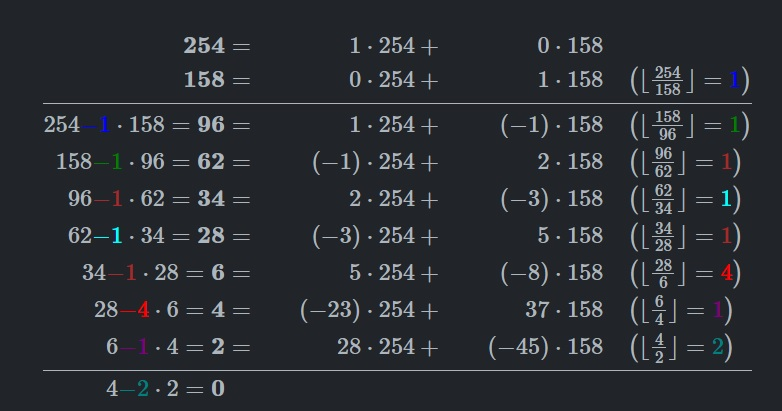
\includegraphics[width=0.6\textwidth]{img/SP-8_0.jpg}
	
	\item \textbf{LDR --- Lineární diofantická rovnice:} libovolná rovnice typu $ax+by=c$, kde $a,b,c \in \mathbb{Z}$ pro 2 neznámé $x, y \in \mathbb{Z}$.
	\begin{itemize}
		\item LDR $ax+by = c$ má alespoň jedno řešení právě tehdy když gcd($a,b$)$\mid c$.
	\end{itemize}
	
	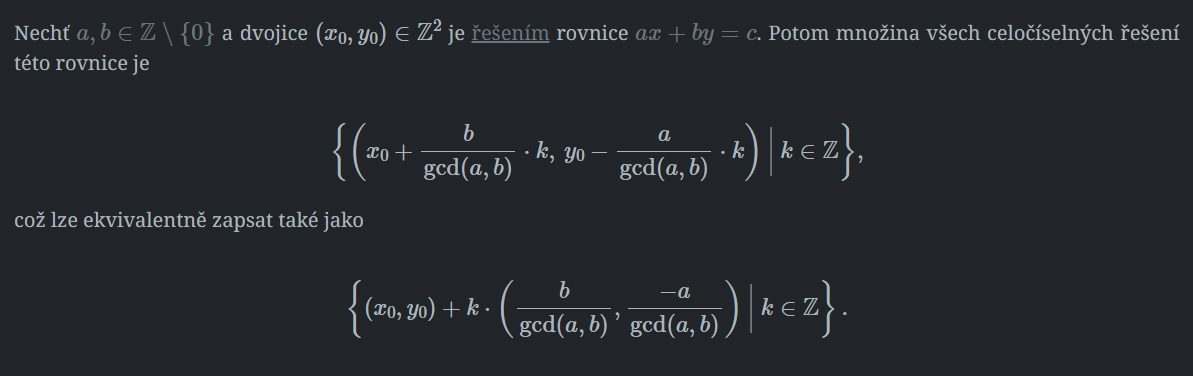
\includegraphics[width=0.9\textwidth]{img/SP-8_1.jpg}
	
	\item Přirozená čísla $\mathbb{N}$ dělíme podle počtu dělitelů do následujících 3 kategorií:
	\begin{itemize}
		\item číslo 1 (1 dělitel --- 1)
		\item \textbf{prvočísla} --- 2 dělitelé, samo číslo a 1
		\item \textbf{složená čísla} --- 3 a více dělitelů
	\end{itemize}
	\newpage
	\item \textbf{Kongruence modulo $m$:} Nechť $a,b \in \mathbb{Z}, m \in \mathbb{N}$. Pokud $m \mid (a - b)$, říkáme že $a$ je kongruentní s $b$ modulo $m$ a píšeme $a \equiv b$ (mod $m$). V opačném případě $a$ není kongruentní s  $b$ modulo $m$ a píšeme $a \not\equiv b$ (mod $m$).
	
	\item \textbf{Množina zbytků:} Nechť $m \geq 2$. Jako $\mathbb{Z}_m$ označíme množinu všech zbytků modulo $m$, $\mathbb{Z}_m = \{0,1,2,...$, $m-1\}$. Operace sčítání: součet a modulo. Násobení totéž.
	
	\item \textbf{Inverze v $\mathbb{Z}_m$:} Aditivní inverze (opačný prvek) --- součet modulo je 0. Multiplikativní inverze (inverzní prvek) --- násobek modulo je 1.
	
	\item \textbf{Existence multiplikativní inverze:} Nechť $m \geq 2$ a $a \in \mathbb{Z}_m$. V $\mathbb{Z}_m$ existuje multiplikativní inverze k $a$ právě tehdy, když gcd($a, m$) = 1. Pokud existuje, je jediná. 
	
	\item \textbf{Krácení v modulu:} Nechť $a, b, c \in \mathbb{Z}$ a $m \in \mathbb{N}, m \geq 2$, označme $d =$ gcd($m, c$). Pak platí ekvivalence: $ac \equiv bc$ (mod $m$) $\Leftrightarrow$ $a \equiv b$ (mod $\frac{m}{d}$)
	
	\item \textbf{Malá Fermatova věta:} Buď $p$ prvočíslo a $a \in \mathbb{N}$ takové přirozené číslo, které není násobkem $p$ (tedy gcd($a, p$) = 1). Potom platí kongruence $a^{p-1} \equiv 1$ (mod $p$).
	
	\item Pokud je $p$ prvočíslo a $a \in \mathbb{Z}_p \land a \neq 0$, pak $a^{p-2}$ je multiplikativní inverzí čísla $a$ mod $p$. 
	
	\item \textbf{Eulerova funkce:} $\varphi$ : $\mathbb{N} \rightarrow \mathbb{N}$ je zobrazení, které každému $n \in \mathbb{N}$ přiřafí počet přirozených čísel menších nebo rovných $n$, která jsou s $n$ nesoudělná. Tedy $(\forall n \in \mathbb{N}(\varphi (n) := |\{k \in \mathbb{N} \mid k \leq n \land$ gcd($k, n$) $ = 1\}|)$.
	
	\item \textbf{Eulerova věta:} Nechť $m \in \mathbb{N}, m \geq 2$ a $a \in \mathbb{N}$ je číslo nesoudělné s $m$. potom platí kongruence $a^{\varphi(m)} \equiv 1$ (mod $m$).
	
	\begin{itemize}
		\item $p$ je prvočíslo, tedy $\varphi(p) = p - 1$
		\item $p$ je prvočíslo, $\alpha \in \mathbb{N}$, pak $\varphi(p^\alpha) = p^\alpha - p^{\alpha - 1}$
		\item $m, n \in \mathbb{N}$, gcd($m, n$) = 1. Potom $\varphi(m\cdot n) = \varphi(m) \cdot \varphi (n)$.
	\end{itemize}
	
	\item Nechť $m \in \mathbb{N}, m \geq 2$ a $a \in \mathbb{Z_m}$ je číslo nesoudělné s $m$. potom $a^{\varphi(m) - 1}$ je multiplikativní inverzí čísla $a$ mod $m$.
	
	\item \textbf{Lineární kongruence:} řešením lineární kongruence rozumíme nalezení všech celých čísel $x$ splňujících kongruenci $ax \equiv b$ (mod $m$), kde $a, b, m \in \mathbb{Z}$ a $m \geq 2$.
	
	\item \textbf{ČVOZ --- Čínská věta o zbytcích}
	
	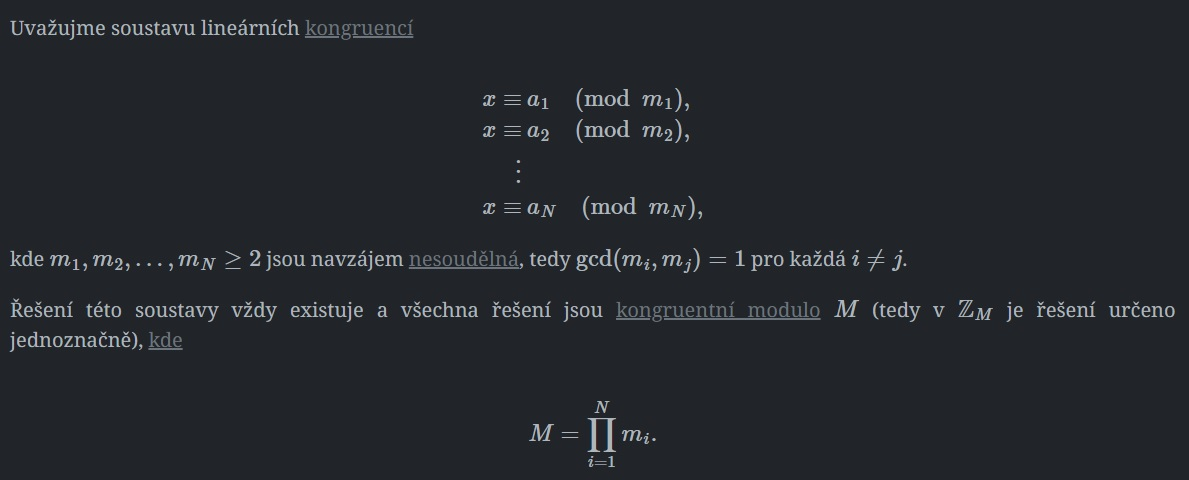
\includegraphics[width=0.9\textwidth]{img/SP-8_2.jpg}
	
	\item Výsledek je: $x = a_1 \cdot M_1 \cdot X_1 + ... + a_N \cdot M_N \cdot X_N$ (mod $M$)
	
	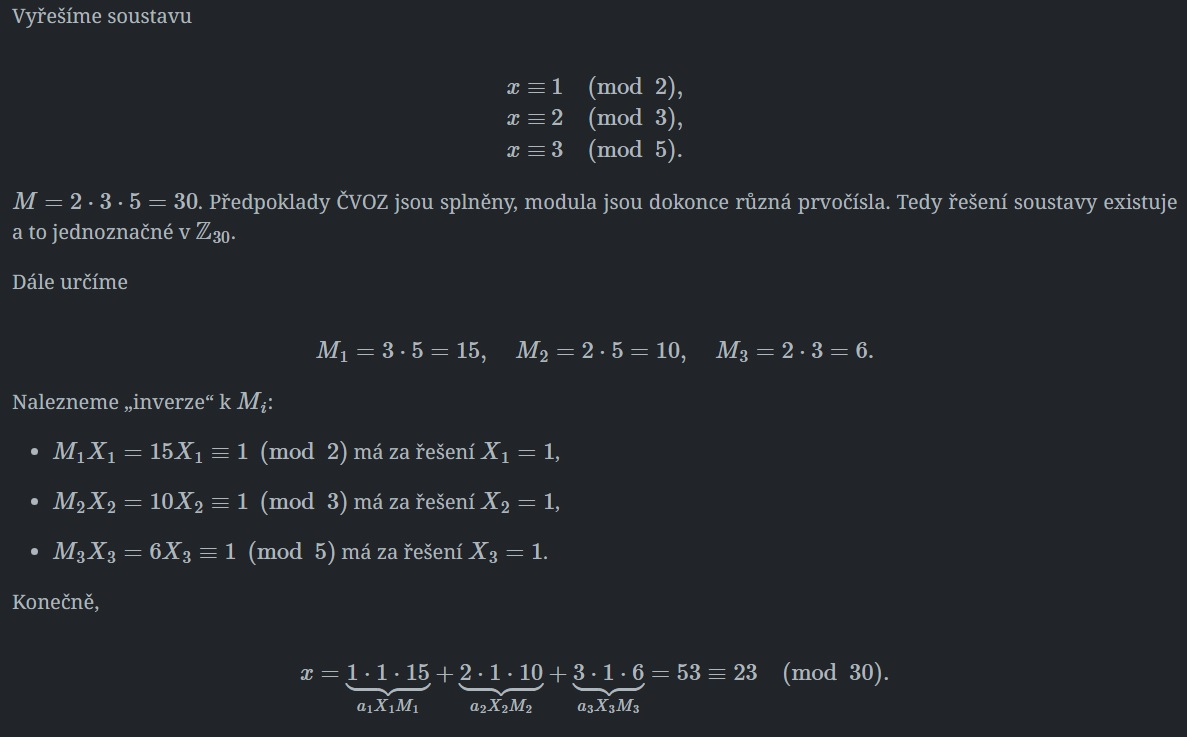
\includegraphics[width=0.9\textwidth]{img/SP-8_3.jpg}
	
	\item \textbf{ZČVOZ --- Zobecněná čínská věta o zbytcích}
	
	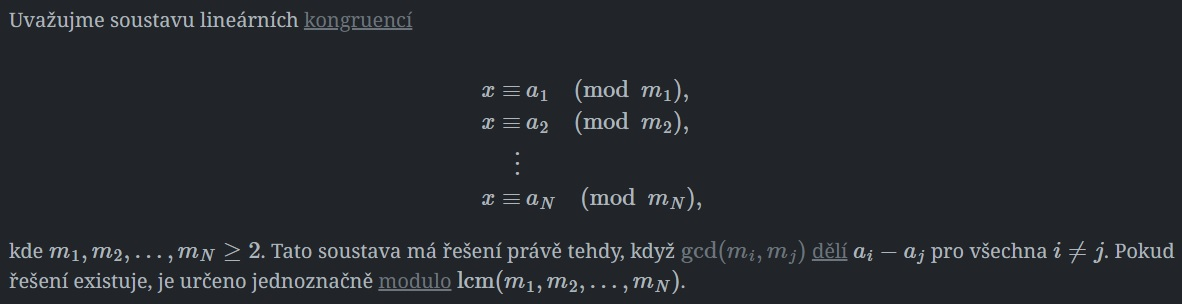
\includegraphics[width=0.9\textwidth]{img/SP-8_4.jpg}
\end{itemize}